% Cover letter: Product Researcher (Product & Design), Pathstream
% CV: Sections/cv_product_researcher_pathstream.tex -> cv_gen/2026-10-30_pathstream/cv_giovanni_tauro-pathstream.pdf
\documentclass[11pt,a4paper,sans]{moderncv}
% Shared preamble and header for the cover letters.
% One main file per application: cl_<company>.tex, built to
% cv_gen/coverletter_giovanni_tauro-<company>.pdf next to cv_giovanni_tauro-<company>.pdf.
% Paths (cl_gen/..., Pictures/...) are relative to the project root, as in the CV (see .latexmkrc).

\moderncvstyle{classic}
\moderncvcolor{blue}

\usepackage[scale=0.80]{geometry}
\setlength{\footskip}{136.00005pt}

\usepackage{fontawesome5}
% hyperref is loaded by moderncv itself; loading it here causes an option clash
\usepackage{xcolor}
\usepackage{graphicx}
\ifxetexorluatex
  \usepackage{fontspec}
  \usepackage{unicode-math}
  \defaultfontfeatures{Ligatures=TeX}
  \setmainfont{Latin Modern Roman}
  \setsansfont{Latin Modern Sans}
  \setmonofont{Latin Modern Mono}
  \setmathfont{Latin Modern Math}
\else
  \usepackage[T1]{fontenc}
  \usepackage{lmodern}
\fi

\usepackage[english]{babel}

% used for the PDF title and the letter closing; the visible header is \clheader below
\name{Giovanni}{Tauro}

% Header: #1 = headline under the name (same as the headline of the matching CV)
\newcommand{\clheader}[1]{%
\noindent
\begin{minipage}[c]{0.74\textwidth}
    {\Huge \textbf{Giovanni Tauro}}\\[-0.2em]
    {\small #1}\\[0.3em]

    \footnotesize
    \faMapMarker*~
    \href{https://www.google.com/maps/search/?api=1&query=Lecco+23900+Italy}
    {\color{blue}Bari-Lecco, Italy}
    \quad
    \faPhone*~
    \href{https://wa.me/393279437161}
    {\color{blue}+39 3279437161}
    \quad
    \faEnvelope~
    \href{mailto:giovanni.taurodi@gmail.com}
    {\color{blue}giovanni.taurodi@gmail.com}
    \\[-0.1em]

    \faLinkedin~
    \href{https://www.linkedin.com/in/giovanni-tauro-gt/}
    {\color{blue}LinkedIn}
    \quad
    \faGithub~
    \href{https://github.com/jotades}
    {\color{blue}GitHub}
    \quad
    \faGraduationCap~
    \href{https://scholar.google.com/citations?user=BS0aVGgAAAAJ&hl=it}
    {\color{blue}Scholar}
    \quad
    \faFilePdf~
    \href{https://www.notion.so/Giovanni-Tauro-2a7901d92f3a800b892af425c5875c6a}
    {\color{blue}Portfolio}
    \quad
    \faCubes~
    \href{https://grabcad.com/giovanni.tauro-3}
    {\color{blue}GrabCAD}

\end{minipage}
\hfill
\begin{minipage}[c]{0.18\textwidth}
    \raggedleft
    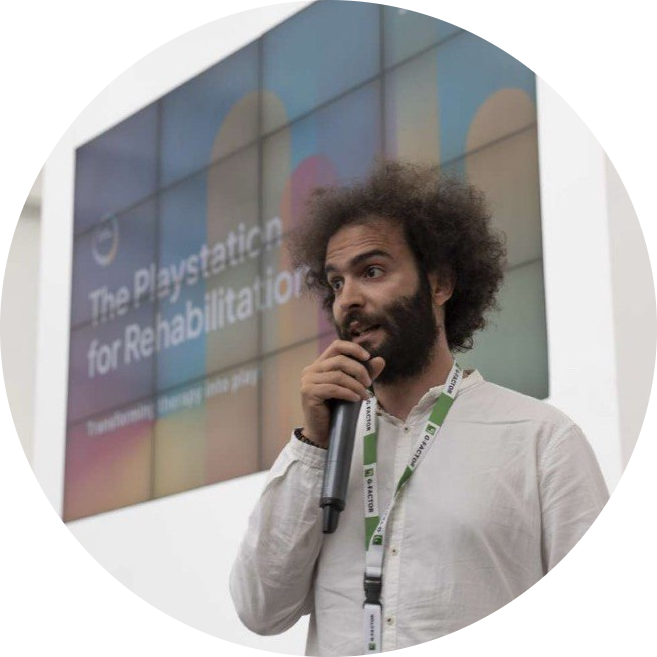
\includegraphics[width=2.8cm]{Pictures/Giovanni_pitch}
\end{minipage}
\vspace{0.1em}
}

\makeatletter
% the sender details are already in \clheader, so skip moderncv's own block
\@detailsfalse
% closing phrase, signature, name
\renewcommand*{\makeletterclosing}{%
  \@closing\\[0.6em]%
  
\includegraphics[height=1.2cm]{Pictures/sign_gt.jpg}\\[0.2em]%
  {\bfseries\@firstname~\@lastname}}
\makeatother


\begin{document}

\clheader{Product Researcher | Discovery, Usability Testing \& Insights}

\recipient{Pathstream}{Product \& Design}
\opening{Dear Pathstream Team,}
\closing{Sincerely,}
\makelettertitle

I am applying for the Product Researcher role in your Product \& Design team. I am Head of Product and co-founder of Rehabilia Technologies, a small startup, and for more than five years I have run user research at CNR-STIIMA, the Italian National Research Council. Helping people grow in the work they already do is close to what I care about, and a role that connects research to both product and curriculum decisions is the kind of work I want to do.

I run research across the whole life of a feature. At Rehabilia, I lead discovery interviews with clinicians, patients and partners, and ongoing field research with clinics and education centres on their pain points, the tools they use and how they decide what to buy, which fed our business plan in the EIT Health bootcamps and the DOHE EdTech accelerator. I test prototypes with users before release and follow them after: our device PhiCube reached a usability score of 85.8/100 (SUS) with 19 children and is now in two multicentre studies with 134 patients. In a small team there is nobody else to run the logistics, so I also coordinate sessions with clinics and partners and keep the people who give us feedback involved.

At CNR-STIIMA, I write study protocols and run usability tests, interviews and questionnaires, from 16 blind participants for an indoor navigation system to children with cerebral palsy for a rehabilitation game, published in the \textit{Italian Journal of Pediatrics}. I have also worked on a serious game for nutritional education, so I know how to check whether a learning experience actually teaches what it should. I analyse the data in Python and Excel and turn it into findings that clinical, engineering and business teams can act on. I use Claude and Claude Code every day to draft, analyse and structure research, and I would enjoy helping build an AI-driven knowledge base.

My users so far have been clinicians, therapists and patients rather than frontline workers in retail or financial services, and I have organised findings with my own structures more than with dedicated repository tools. Clinicians and therapists are frontline staff too, though, and the skills carry over: listening carefully, working from limited information and turning what people say into decisions a team can trust.

I would welcome the chance to talk about how I could contribute.

\makeletterclosing

\end{document}
